\documentclass[11pt,a4paper]{article}

\usepackage[utf8]{inputenc}
\usepackage[margin=1in]{geometry}
\usepackage{graphicx}
\usepackage{amsmath,amssymb}
\usepackage{booktabs}
\usepackage{float}
\usepackage{caption}
\usepackage{microtype}
\usepackage{titlesec}
\usepackage{parskip}
\usepackage{hyperref}

\hypersetup{
    colorlinks=true,
    linkcolor=blue,
    citecolor=blue,
    urlcolor=blue
}

% Section styling to match rigorous academic reports
\titleformat{\section}{\large\bfseries}{\thesection}{1em}{}
\titleformat{\subsection}{\normalsize\bfseries}{\thesubsection}{1em}{}
\titleformat{\subsubsection}{\small\bfseries}{\thesubsubsection}{1em}{}

\setlength{\parindent}{0pt}
\setlength{\parskip}{6pt}

\begin{document}

% --- TITLE BLOCK ---
\begin{center}
    {\Large \textbf{CARNEGIE MELLON UNIVERSITY-AFRICA}}\\[4pt]
    {\large \textbf{Data, Inference \& Applied Machine Learning}}\\[2pt]
    {\textbf{Course 18-785 --- Assignment 3}}\\[8pt]
    \textbf{Ndizeye Alain} \quad (\textbf{Andrew ID: nalain})\\[4pt]
    \today
\end{center}

\newpage

% --- LIBRARIES PAGE ---
\subsection*{Libraries Used}
\texttt{numpy}, \texttt{pandas}, \texttt{scipy.stats}, \texttt{matplotlib.pyplot}, \texttt{openpyxl}, \texttt{urllib.request}, \texttt{json}

\newpage

% ==========================================
% QUESTION 1
% ==========================================
\section*{Question 1: Speed of Light (Michelson's 1879 Experiment)}

\subsection*{Steps / Explanation}
Michelson's 1879 experiment measured the speed of light in air across an Annapolis baseline of approximately 2,000 feet using revolving mirrors. Twenty determinations were loaded from the baseline JSON file to test against the accepted benchmark $\mu_0 = 299,734.50\text{ km/s}$ at $\alpha = 0.05$. Distributional normality was visually evaluated via histogram and Q-Q plot and statistically tested using the Shapiro-Wilk test ($W$-statistic). A two-tailed one-sample $t$-test ($df = 19$) was conducted to compute sample mean, standard error ($\text{SEM} = s / \sqrt{n}$), critical values ($\pm t_{\text{crit}}$), complete rejection intervals, 95\% CI, and $p$-value. Finally, absolute and percentage bias were quantified alongside an $n = 200$ counterfactual.

\subsection*{Results}

\subsubsection*{(a) Null and Alternative Hypotheses:}
\begin{figure}[H]
    \centering
    
\includegraphics[width=0.75\textwidth]{images/q1a_hypotheses.png}
\end{figure}

\subsubsection*{(b) Normality Assessment (Shapiro-Wilk Test and Visual Diagnostics):}
\begin{figure}[H]
    \centering
    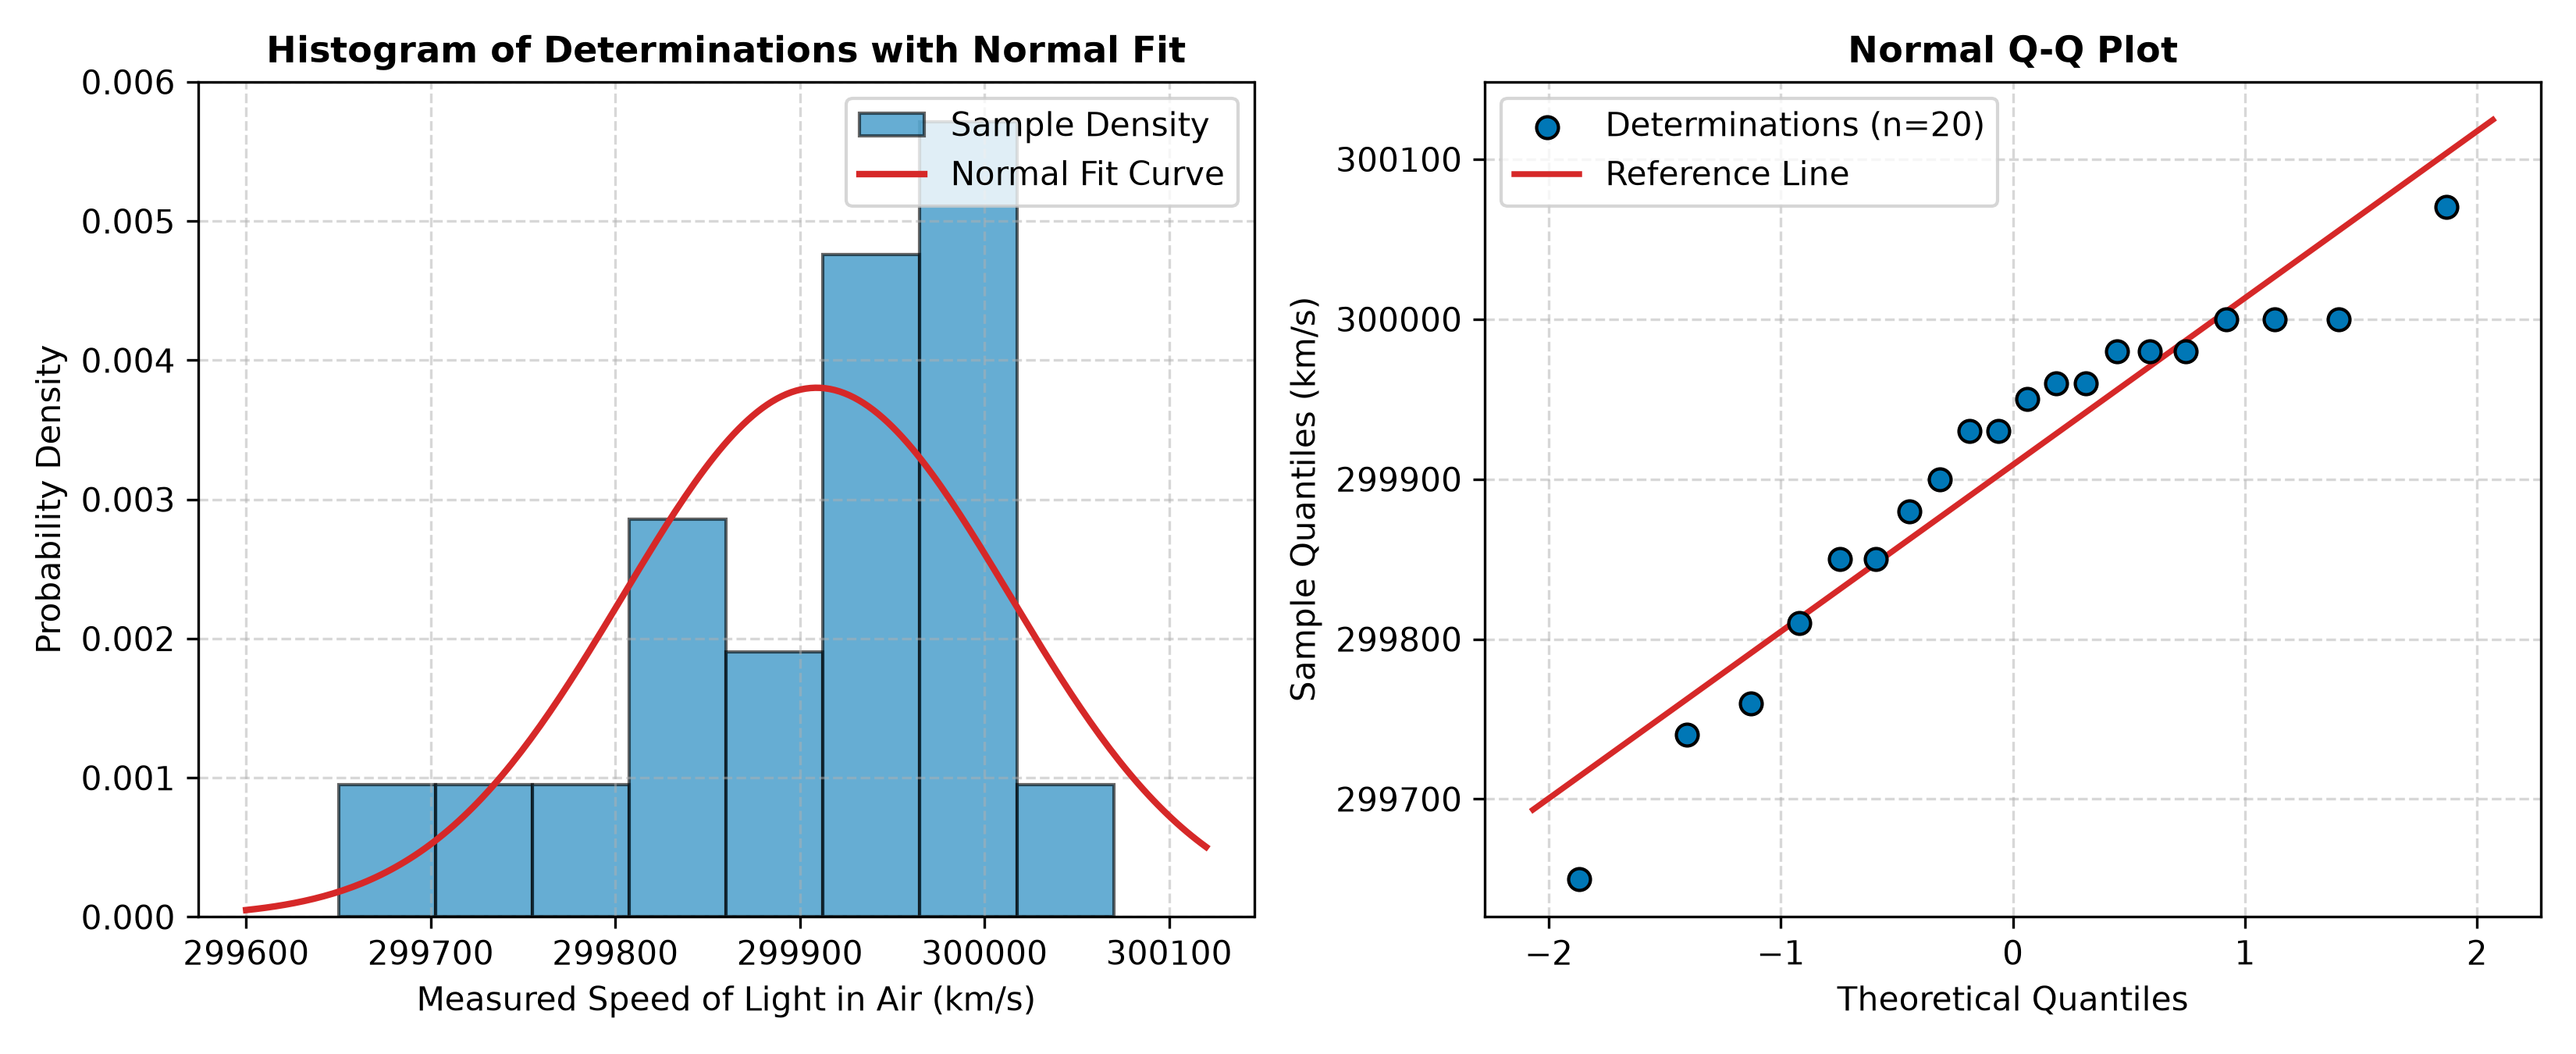
\includegraphics[width=0.95\textwidth]{images/fig1_normality_diagnostics.png}
    \caption{Distributional normality diagnostics for Michelson's 1879 speed of light determinations (Histogram with theoretical normal fit and Normal Q-Q plot).}
\end{figure}

\begin{figure}[H]
    \centering
    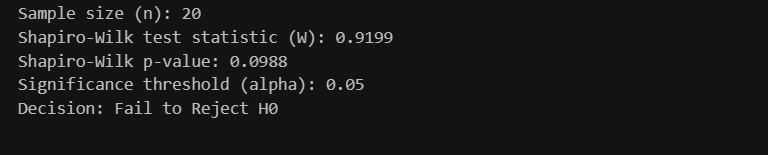
\includegraphics[width=0.75\textwidth]{images/q1b_normality.png}
\end{figure}

\subsubsection*{(c) One-Sample $t$-Test Results and Complete Statistical Intervals:}
\begin{figure}[H]
    \centering
    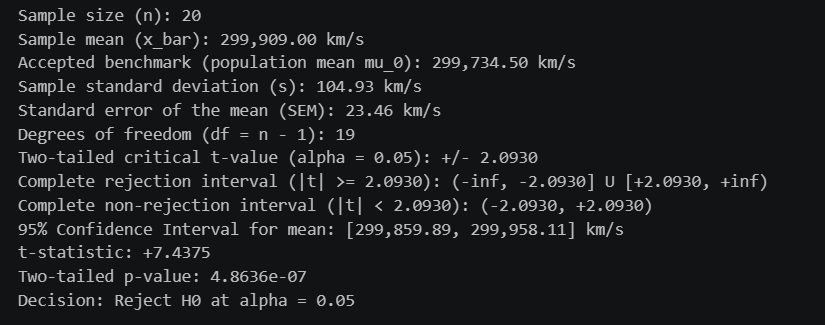
\includegraphics[width=0.85\textwidth]{images/q1c_ttest.png}
\end{figure}

\subsubsection*{(d) Measurement Bias and Counterfactual $n = 200$ Evaluation:}
\begin{figure}[H]
    \centering
    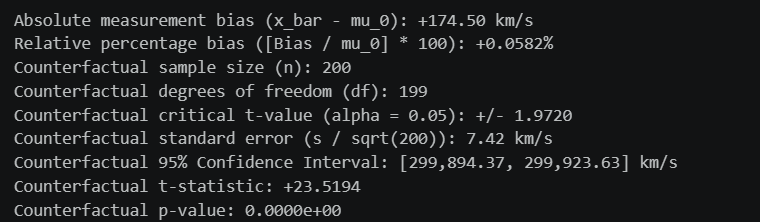
\includegraphics[width=0.80\textwidth]{images/q1d_bias.png}
\end{figure}

\subsection*{Interpretation}

\textbf{(a) Choice of Hypothesis and Tail Justification:} A two-tailed test ($H_0: \mu = \mu_0$ vs. $H_1: \mu \neq \mu_0$) was selected because physical measurement errors could plausibly deviate bidirectionally from the true constant. Optical misalignment, mirror timing drift, baseline surveying errors, or atmospheric temperature fluctuations could cause measured velocity to either overestimate or underestimate the true speed. Symmetrical rejection regions ($\alpha/2 = 0.025$ in each tail) prevent directional bias.

\textbf{(b) Normality Assessment and Consequences of Violation:} With $n = 20$, the Central Limit Theorem cannot guarantee normality, necessitating the Shapiro-Wilk test. The result ($W = 0.9199, p = 0.0988 > 0.05$) fails to reject $H_0$, confirming normality is statistically sound for parametric testing. Both visual diagnostics in Figure 1 support this conclusion: the histogram displays approximate bell-shaped symmetry around the sample mean ($299,909\text{ km/s}$), and determinations in the Q-Q plot adhere closely to the theoretical diagonal line without extreme curvilinear departure or heavy tails. If normality were violated by heavy skewness or severe outliers, standard errors and $t$-distribution critical values would be distorted, requiring non-parametric alternatives such as the Wilcoxon signed-rank test.

\textbf{(c) Significance Test Conclusion and Confidence Interval:} The sample mean ($\bar{x} = 299,909.00\text{ km/s}, \text{SEM} = 23.46\text{ km/s}$) yields $t = +7.4375$ on $df = 19$, falling far into the rejection region $(-\infty, -2.0930] \cup [+2.0930, +\infty)$ with $p = 4.86\times 10^{-7}$. Furthermore, the accepted benchmark ($299,734.50\text{ km/s}$) lies $125.40\text{ km/s}$ below the 95\% confidence interval $[299,859.90, 299,958.10]\text{ km/s}$. The null hypothesis is rejected, demonstrating that Michelson's measurements systematically deviate from the accepted benchmark due to instrumentation calibration bias rather than random variation.

\textbf{(d) Scientific Importance vs. Statistical Significance and Counterfactual Insight:} Although statistically significant, the $+174.50\text{ km/s}$ bias represents just $+0.0582\%$ relative error---an extraordinary $>99.94\%$ accuracy for 1879 mechanical instrumentation. Under the $n = 200$ counterfactual, SEM contracts from $23.46\text{ km/s}$ to $7.42\text{ km/s}$ ($t = +23.52, p < 10^{-50}$), narrowing the 95\% CI to $[299,894.37, 299,923.63]\text{ km/s}$. This demonstrates that expanding sample size tightens precision around the sample mean, but cannot remove systematic physical calibration errors.

\newpage
% ==========================================
% QUESTION 2
% ==========================================
\section*{Question 2: Chick Weights (Feed Types: Casein vs. Soybean)}

\subsection*{Steps / Explanation}
Six-week chick weights were analyzed across two nutritional diets (Casein vs. Soybean) from Snedecor (1948) using CSV data ($N = 26$). Group sample sizes, means, standard deviations, and variances were computed. Because sample variances were heterogeneous ($s_1^2/s_2^2 = 1.42$), a two-tailed hypothesis ($H_0: \mu_1 = \mu_2$ vs. $H_1: \mu_1 \neq \mu_2$) was formulated and Welch's unequal-variance $t$-test was applied using Welch-Satterthwaite degrees of freedom, reporting test statistics, complete rejection intervals, 95\% CI, and Cohen's $d$ effect size alongside a comparative boxplot.

\subsection*{Results}

\subsubsection*{(a) Statistical Hypotheses and Test Classification:}
\begin{figure}[H]
    \centering
    \includegraphics[width=0.70\textwidth]{images/q2a_hypotheses.png}
\end{figure}

\subsubsection*{(b) Descriptive Summary Statistics (Sample Sizes Stated in Text):}
\begin{figure}[H]
    \centering
    \includegraphics[width=0.75\textwidth]{images/q2b_descriptive.png}
\end{figure}

\subsubsection*{(c) Welch's Two-Sample $t$-Test Results and Complete Statistical Intervals:}
\begin{figure}[H]
    \centering
    \includegraphics[width=0.80\textwidth]{images/q2c_welch.png}
\end{figure}

\subsubsection*{(d) Practical Effect Size:}
\begin{figure}[H]
    \centering
    \includegraphics[width=0.70\textwidth]{images/q2d_effect_size.png}
\end{figure}

\subsubsection*{(e) Distributional Boxplot Comparison:}
\begin{figure}[H]
    \centering
    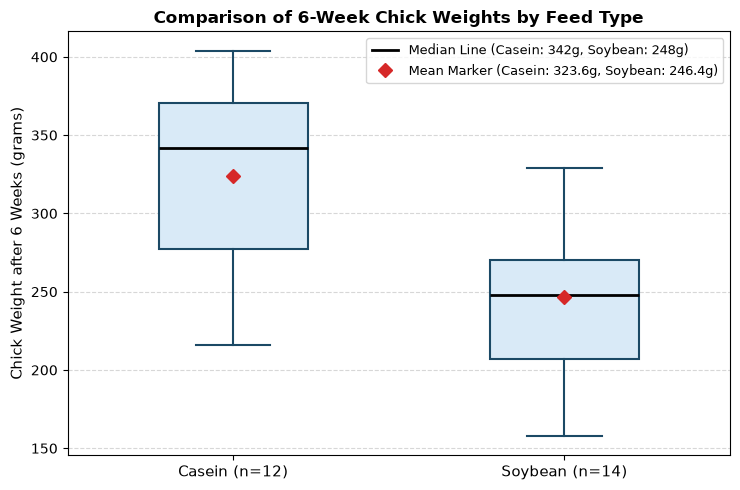
\includegraphics[width=0.82\textwidth]{images/fig1_chick_weights_boxplot.png}
    \caption{Six-week chick weight distribution under Casein vs. Soybean feed diets.}
\end{figure}

\subsection*{Interpretation}

\textbf{(a) Test Design Justification and Method Choice:} The hypotheses tested were $H_0: \mu_{\text{casein}} = \mu_{\text{soybean}}$ vs. $H_1: \mu_{\text{casein}} \neq \mu_{\text{soybean}}$ at $\alpha = 0.05$. An independent two-sample test was required because chicks were randomly allocated into distinct, mutually exclusive dietary cohorts with no biological pairing. A two-tailed test guards against either feed underperforming. Welch's unequal-variance $t$-test was selected over Student's $t$-test because group variances were unequal ($4151.72\text{ g}^2$ vs. $2929.96\text{ g}^2$), preventing inflated Type I error rates.

\textbf{(b) Descriptive Findings:} The sample comprises $N = 26$ chicks ($n_1 = 12$ Casein, $n_2 = 14$ Soybean). Casein achieved a substantially higher mean ($\bar{x}_1 = 323.58\text{ g}, s_1 = 64.43\text{ g}$) than Soybean ($\bar{x}_2 = 246.43\text{ g}, s_2 = 54.13\text{ g}$). The variance ratio $s_1^2/s_2^2 = 1.42$ reflects substantial heteroscedasticity driven by greater individual growth variation within the Casein cohort, empirically validating the selection of Welch's $t$-test.

\textbf{(c) Welch Test Significance and Confidence Interval:} Welch's test produced $t = +3.2743$ ($df = 21.63, p = 0.0035$), falling into the upper rejection region $[+2.0759, +\infty)$ at $\alpha = 0.05$. The difference in means ($+77.15\text{ g}, \text{SE}_{\text{diff}} = 23.56\text{ g}$) has a 95\% CI of $[+28.24\text{ g}, +126.07\text{ g}]$, strictly excluding zero. Because $p < 0.01$, $H_0$ is rejected; random variation has only a 0.35\% probability of producing this gap, confirming a statistically significant weight advantage for Casein.

\textbf{(d) Practical Agricultural Importance vs. Statistical Significance:} The $+77.15\text{ g}$ gain represents a $+31.3\%$ weight advantage and a standardized effect size of Cohen's $d = 1.31$, indicating massive biological importance. However, commercial poultry adoption requires evaluating Feed Conversion Ratios ($\text{FCR} = \text{kg feed} / \text{kg gain}$) and feed market costs per ton. Because purified casein protein is far more expensive than commercial soybean meal, adoption is only profitable if faster broiler turnaround offsets higher feed acquisition costs.

\textbf{(e) Boxplot Features:} Figure 2 corroborates the statistical findings directly. The Casein median ($342\text{ g}$) and mean ($323.6\text{ g}$) exceed the entire 75th percentile ($\sim 271\text{ g}$) of the Soybean group, showing minimal interquartile overlap. Both distributions display symmetric spreads with no extreme outliers, confirming that Casein's advantage represents a systematic upward shift across the entire cohort distribution rather than an artifact of outlier birds.

\newpage
% ==========================================
% QUESTION 3
% ==========================================
\section*{Question 3: Global Demographics (Fertility Rate vs. GDP per Capita PPP, 2024)}

\subsection*{Steps / Explanation}
Data was queried directly via the World Bank API for 2024 indicator codes \texttt{SP.DYN.TFRT.IN} (Fertility Rate) and \texttt{NY.GDP.PCAP.PP.CD} (GDP per Capita PPP). To eliminate geopolitical distortion, the sample was restricted to 183 reporting sovereign UN Member States. A dual-panel scatter plot comparing linear and logarithmic GDP scales was generated with a 2.1 replacement line, Pearson correlations were estimated on raw and log-transformed GDP alongside Spearman rank correlation, extreme observations were identified using a standardized $|z| > 2.5$ threshold, and all three correlations were recomputed on trimmed data ($n = 177$) to evaluate sensitivity.

\subsection*{Results}

\subsubsection*{(a) Linear vs. Logarithmic Scatter Plot Comparison and Valid Country Count in Text:}
\begin{figure}[H]
    \centering
    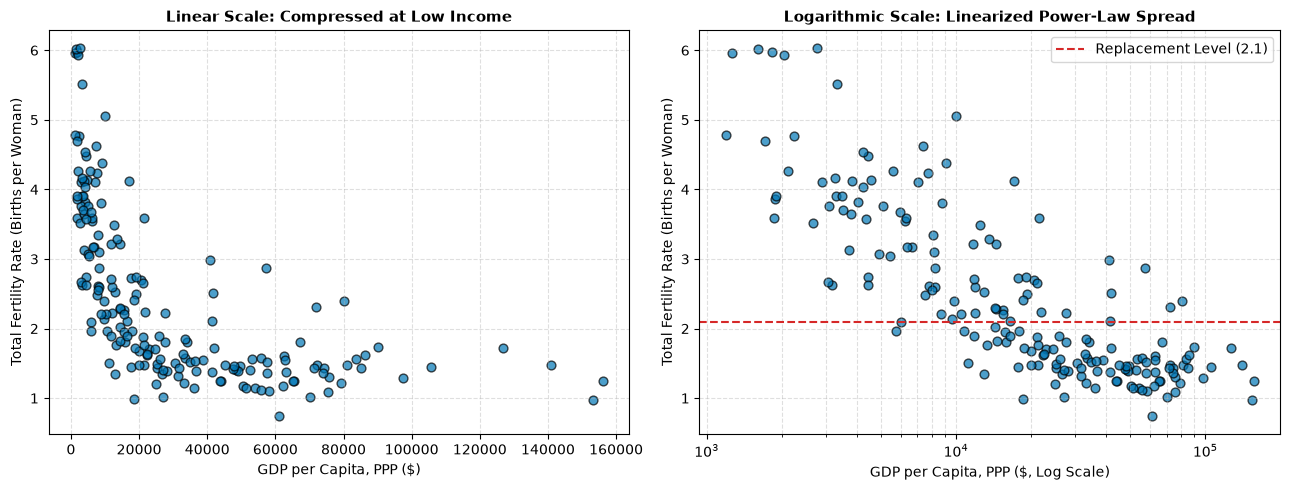
\includegraphics[width=0.98\textwidth]{images/fig2_fertility_gdp_scatter.png}
    \caption{Global Total Fertility Rate vs. GDP per Capita, PPP (2024) across 183 UN Member States (Linear vs. Logarithmic Scale Comparison with 2.1 Replacement Level).}
\end{figure}

\begin{figure}[H]
    \centering
    \includegraphics[width=0.75\textwidth]{images/q3a_countries_count.png}
\end{figure}

\subsubsection*{(b) Complete Correlation Analysis on Full Sovereign Sample ($n = 183, df = 181$):}
\begin{figure}[H]
    \centering
    \includegraphics[width=0.85\textwidth]{images/q3b_correlation.png}
\end{figure}

\subsubsection*{(c) Outlier Identification ($|z| > 2.5$) and Robustness Trimmed Sample ($n = 177, df = 175$):}
\begin{figure}[H]
    \centering
    \includegraphics[width=0.90\textwidth]{images/q3c_outliers.png}
\end{figure}

\subsection*{Interpretation}

\textbf{(a) Methodological Choice of Axis Scale (Linear vs. Logarithmic):} A logarithmic horizontal axis was selected because global GDP per capita is severely right-skewed, spanning orders of magnitude from under \$1,500 (e.g., Central African Republic) to over \$120,000 (e.g., Luxembourg). A linear scale bunches developing nations against the axis while isolating wealthy economies as extreme leverage points. Logarithmic scaling linearizes the power-law relationship, equalizing visual variance and displaying proportional economic growth across nations uniformly.

\textbf{(b) Full Correlation Analysis and Why the Correlation is Negative:} All three metrics reveal a decisive, highly significant negative relationship ($p < 10^{-18}$): Pearson on raw GDP ($r = -0.6004$), Pearson on $\log(\text{GDP})$ ($r = -0.8223$), and Spearman rank ($\rho = -0.8206$). The $0.2219$ increase in Pearson $r$ upon log-transformation and its alignment with Spearman $\rho$ confirms a non-linear power-law decay. This negative correlation is driven by rising female educational opportunity costs, parental quality-quantity trade-offs, lower child mortality, and state pensions.

\textbf{(c) Outlier Observations and Sensitivity Analysis:} Applying $|z| > 2.5$ flagged six high-fertility low-income nations: Chad ($z = +2.96$), Somalia ($z = +2.95$), DR Congo ($z = +2.93$), Central African Republic ($z = +2.90$), Niger ($z = +2.89$), and Mali ($z = +2.54$). Trimming these six ($n = 177, df = 175$) shifted Pearson $\log(\text{GDP})$ from $-0.8223$ to $-0.8051$ and Spearman from $-0.8206$ to $-0.8030$ ($\Delta < 0.02$). This minimal sensitivity demonstrates that the negative fertility-income link is an exceptionally robust global empirical regularity.

\textbf{(d) Limitations of Single-Year Cross-Sectional Data and the Panel Solution:} Single-year 2024 data captures between-country correlations at one point in time, confounding income effects with unobserved cultural, religious, and institutional factors (omitted variable bias) while risking reverse causality. A longitudinal panel framework tracking countries over multiple decades resolves this by using country fixed effects to control for time-invariant national heterogeneity and year fixed effects to absorb global shocks, identifying true causal dynamics.

\newpage
% ==========================================
% QUESTION 4
% ==========================================
\section*{Question 4: UK House Price Index Time Series Analysis (Nationwide 1991–2026)}

\subsection*{Steps / Explanation}
Nationwide's UK monthly average house price series was analyzed from Jan 1991 to Aug 2026 ($N = 428$ months) using OpenPyXL. The price series was plotted with an overlaid 12-month rolling moving average to isolate long-term trend from monthly noise and identify macroeconomic regimes. Twelve-month YoY percentage change was computed against a 0\% baseline to identify peak growth and trough decline, monthly return autocorrelations were analyzed for lags 1--40 with 95\% Bartlett bounds ($\pm 1.96 / \sqrt{N}$), and Geometric CAGR was calculated across historical epochs.

\subsection*{Results}

\subsubsection*{(a) Full Time Series with 12-Month Moving Average Overlay (Sample Span in Text):}
The dataset covers exactly 428 continuous monthly observations from January 1991 (\pounds 53,051.72) to August 2026 (\pounds 275,465.06).

\begin{figure}[H]
    \centering
    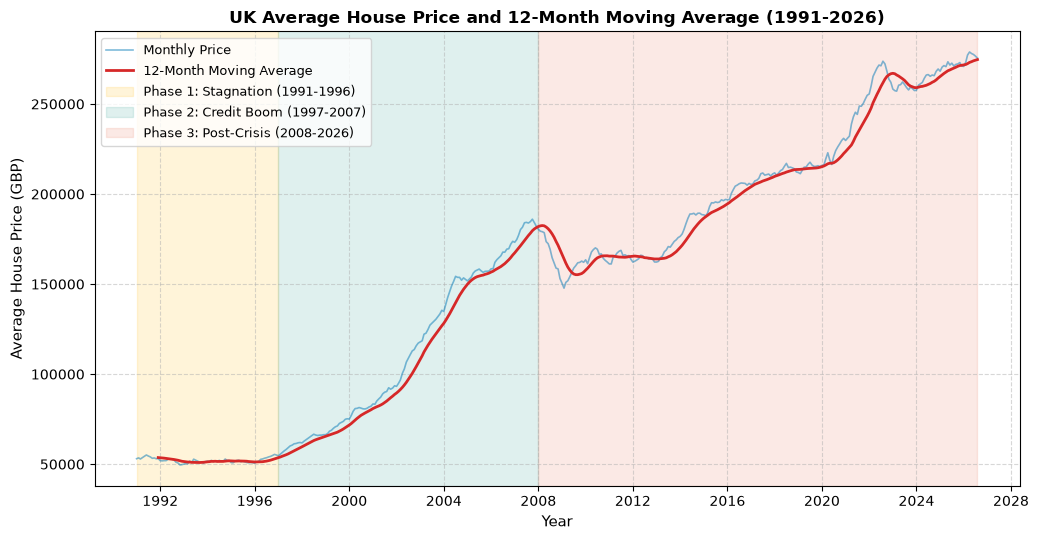
\includegraphics[width=0.95\textwidth]{images/fig3_uk_housing_timeseries.png}
    \caption{UK Average House Price Time Series and 12-Month Moving Average with Three Macroeconomic Regimes (Jan 1991 -- Aug 2026).}
\end{figure}

\begin{figure}[H]
    \centering
    \includegraphics[width=0.75\textwidth]{images/q4a_span.png}
\end{figure}

\subsubsection*{(b) Year-on-Year Growth Dynamics and Exact Historical Extremes:}
\begin{figure}[H]
    \centering
    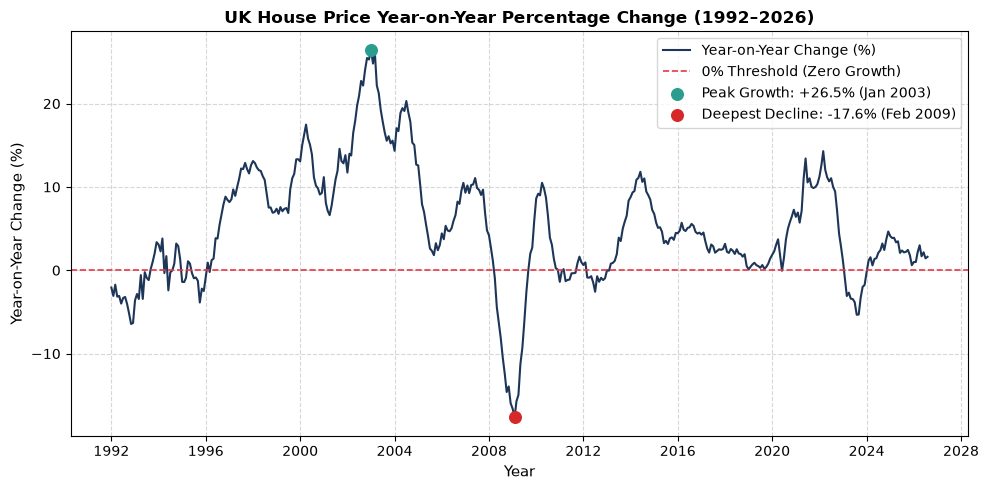
\includegraphics[width=0.95\textwidth]{images/fig4_uk_housing_yoy.png}
    \caption{UK House Price Year-on-Year Percentage Change with 0\% Threshold and Historical Extremes (1992--2026).}
\end{figure}

\begin{figure}[H]
    \centering
    \includegraphics[width=0.75\textwidth]{images/q4b_extremes.png}
\end{figure}

\subsubsection*{(c) Autocorrelation Function (ACF) of Monthly Returns (Lags 1–40):}
\begin{figure}[H]
    \centering
    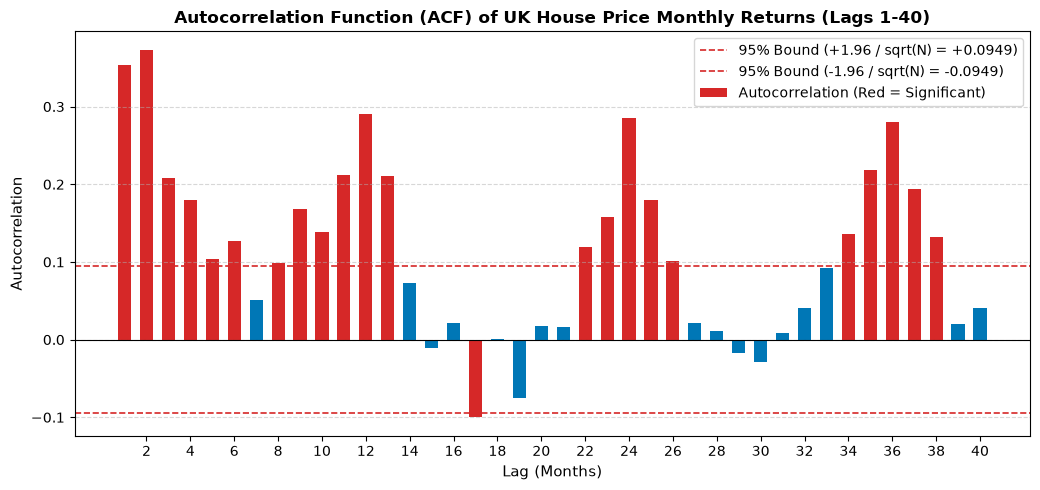
\includegraphics[width=0.95\textwidth]{images/fig5_uk_housing_acf.png}
    \caption{Sample Autocorrelation Function (ACF) of UK House Price Monthly Returns with 95\% Bartlett Bounds (Red Bars Indicate Significant Lags).}
\end{figure}

\begin{figure}[H]
    \centering
    \includegraphics[width=0.75\textwidth]{images/q4c_acf.png}
\end{figure}

\subsubsection*{(d) Compound Annual Growth Rate (CAGR) Across Historical Epochs:}
\begin{figure}[H]
    \centering
    \includegraphics[width=0.85\textwidth]{images/q4d_cagr.png}
\end{figure}

\subsection*{Interpretation}

\textbf{(a) Market Trend and Three Distinct Historical Phases:} The time series displays three distinct macroeconomic regimes: (1) Post-1990s Stagnation \& Recovery (1991--1996), characterized by high base interest rates, negative equity, and slow recovery following the ERM exit; (2) Credit \& Mortgage Boom (1997--2007), driven by aggressive bank lending, buy-to-let deregulation, and economic expansion; and (3) Post-Financial Crisis Regime (2008--2026), marked by the 2008 liquidity crunch, Bank of England zero-rate stimulus, COVID stamp-duty holidays, and subsequent rate hikes.

\textbf{(b) Alignment of Growth Extremes:} The two YoY extremes align perfectly with the macroeconomic epochs in part (a). The historical peak of $+26.47\%$ occurred in January 2003 during the height of the pre-crisis credit expansion, fueled by 100\%+ loan-to-value mortgages and lax underwriting. The deepest contraction of $-17.63\%$ occurred in February 2009 during the Global Financial Crisis, when Northern Rock collapsed, wholesale bank funding froze, and mortgage lending ground to a halt.

\textbf{(c) Autocorrelation Pattern and Bartlett Threshold Justification:} The Bartlett 95\% white-noise bounds are $\pm 1.96 / \sqrt{427} = \pm 0.0949$. Lags 1 ($+0.3532$) and 2 ($+0.3733$) significantly breach the upper bound, reflecting substantial short-term momentum. This persistence stems from real estate microstructure: backward-looking appraisals, seller asking-price stickiness, and long transaction delays. Additionally, lag 12 ($+0.2901$) is highly significant, capturing strong annual seasonality associated with the spring buying cycle.

\textbf{(d) Methodological Choice on Period Splitting:} Splitting the timeline at 2008 provides a far more informative economic picture than reporting only the full-period CAGR (4.74\%). Pre-2008 annualized growth reached an extraordinary 7.56\% per year, whereas post-2008 growth dropped to 2.24\% per year---barely outpacing inflation. The 2008 crash represented a permanent structural break in real estate finance due to strict mortgage stress-testing and regulatory capital rules, making a single full-period rate a misleading blended figure.

\newpage
% ==========================================
% QUESTION 5
% ==========================================
\section*{Question 5: UK House Prices vs. FTSE 100 Index (1991–2026)}

\subsection*{Steps / Explanation}
Monthly UK house prices were merged with the FTSE 100 equity index over 428 continuous months (Jan 1991 to Aug 2026). The closing price column (\texttt{Close}) was selected from \texttt{FTSE100.csv} to compute returns. Both series were normalized to base 100 in Jan 1991 and plotted on a dual time-series graph. Multi-year performance was evaluated using Geometric CAGR and annualized arithmetic mean returns, quantifying compounding volatility drag ($\approx 0.5 \sigma^2$). Finally, sample standard deviations of monthly returns were annualized via the $\sqrt{12}$ rule to compare volatility ratios.

\subsection*{Results}

\subsubsection*{(a) Normalized Dual Time Series Comparison (Jan 1991 = 100, 428 Months in Text):}
The synchronized dataset spans exactly 428 continuous months from January 1991 to August 2026.

\begin{figure}[H]
    \centering
    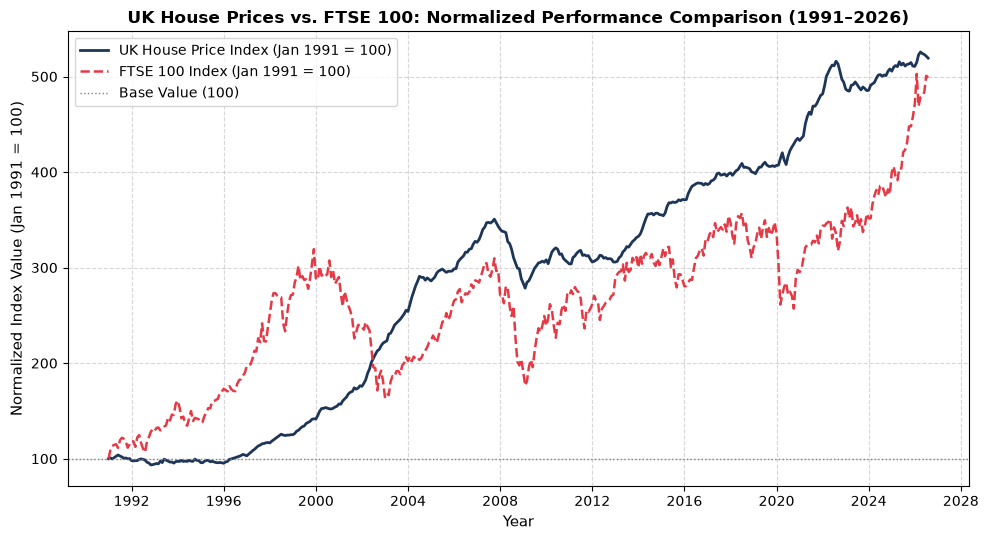
\includegraphics[width=0.95\textwidth]{images/fig6_housing_vs_ftse.png}
    \caption{Normalized Capital Performance of UK House Prices vs. FTSE 100 Index (Jan 1991 = 100).}
\end{figure}

\begin{figure}[H]
    \centering
    \includegraphics[width=0.75\textwidth]{images/q5a_span.png}
\end{figure}

\subsubsection*{(b) Annualized Return Comparison (35.58 Years, 427 Monthly Intervals):}
\begin{figure}[H]
    \centering
    \includegraphics[width=0.80\textwidth]{images/q5b_returns.png}
\end{figure}

\subsubsection*{(c) Annualized Volatility and Risk Comparison:}
\begin{figure}[H]
    \centering
    \includegraphics[width=0.80\textwidth]{images/q5c_volatility.png}
\end{figure}

\subsection*{Interpretation}

\textbf{(a) Normalized Performance Comparison:} Figure 7 compares capital growth over 35.58 years: normalized housing appreciated to 519.24 ($+419.24\%$) while the FTSE 100 reached 498.75 ($+398.75\%$). While residential housing experienced a smooth, steady upward trajectory with only one major drawdown in 2008, the equity index endured violent boom-bust cycles---surging in the dot-com bubble, crashing in 2002 and 2008, and suffering prolonged lost decades before regaining its previous highs.

\textbf{(b) Methodological Choice between Geometric CAGR and Arithmetic Mean (Volatility Drag):} For multi-year capital compounding, Geometric CAGR (4.62\% for FTSE, 4.74\% for Housing) is the only mathematically sound metric. Arithmetic mean returns (5.43\% for FTSE) severely overstate investor wealth accumulation because they ignore compounding losses: $\text{CAGR} \approx \mu_{\text{arith}} - 0.5 \sigma^2$. High equity volatility generates a substantial $-0.81\%$ annual drag, whereas low housing volatility produces negligible drag ($-0.03\%$), making arithmetic averages inappropriate for multi-year horizons.

\textbf{(c) Volatility Scaling and the Return-Risk Comparison:} Annualized volatility for the FTSE 100 is 13.38\% ($s = 3.86\%$ monthly), compared to just 3.67\% ($s = 1.06\%$ monthly) for housing, yielding a $3.65\times$ risk ratio. The asset with higher risk did not deliver higher returns---the FTSE delivered lower capital CAGR (4.62\% vs. 4.74\%) despite carrying 365\% higher volatility. This violates classical Capital Asset Pricing theory, showing that public equities carried massive uncompensated volatility risk relative to housing.

\textbf{(d) Which Was the Better Investment? Missing Factors in the Comparison:} Grounded in the computed results, housing achieved superior risk-adjusted capital returns (4.74\% CAGR at 3.67\% volatility vs. 4.62\% at 13.38\%). However, declaring housing the definitively superior investment remains incomplete because critical cash-flow and friction factors are omitted. First, the comparison ignores income: housing generates gross rental yields ($\sim 4\text{--}6\%$), while the FTSE price index excludes reinvested dividends ($\sim 3\text{--}4\%$), which would dramatically boost total equity returns. Second, housing benefits from mortgage leverage but incurs heavy transaction, stamp duty, and maintenance costs, unlike frictionless liquid stocks.

\newpage
% ==========================================
% REFERENCES
% ==========================================
\section*{References}

\begin{enumerate}
    \item[{[1]}] A. A. Michelson, ``Experimental determination of the velocity of light made at the U.S. Naval Academy, Annapolis,'' \emph{Astronomical Papers Prepared for the Use of the American Ephemeris and Nautical Almanac}, vol. 1, pp. 115--144, 1879.
    \item[{[2]}] G. W. Snedecor, \emph{Statistical Methods Applied to Experiments in Agriculture and Biology}, 4th ed. Ames, IA: Iowa State College Press, 1948.
    \item[{[3]}] World Bank Group, ``Fertility rate, total (births per woman),'' \emph{World Bank Open Data}, Indicator SP.DYN.TFRT.IN, 2024. [Online]. Available: \url{https://data.worldbank.org/indicator/SP.DYN.TFRT.IN}
    \item[{[4]}] World Bank Group, ``GDP per capita, PPP (current international \$),'' \emph{World Bank Open Data}, Indicator NY.GDP.PCAP.PP.CD, 2024. [Online]. Available: \url{https://data.worldbank.org/indicator/NY.GDP.PCAP.PP.CD}
    \item[{[5]}] United Nations, ``Member States of the United Nations,'' \emph{United Nations Department of Global Communications}, 2024. [Online]. Available: \url{https://www.un.org/en/about-us/member-states}
    \item[{[6]}] Nationwide Building Society, ``UK House Price Index Data Library: Monthly Indices (Post-1991),'' \emph{Nationwide Research}, 2026. [Online]. Available: \url{https://www.nationwidehousepriceindex.co.uk}
    \item[{[7]}] FTSE Russell / Yahoo Finance, ``FTSE 100 Index Historical Monthly Price Data (\^{}FTSE),'' \emph{London Stock Exchange Group}, 2026. [Online]. Available: \url{https://finance.yahoo.com/quote/%5EFTSE}
    \item[{[8]}] Barclays, \emph{Barclays Equity Gilt Study: 124 Years of UK Asset Class Returns}, Barclays Investment Bank Research, London, UK, 2024.
\end{enumerate}

\end{document}
